\documentclass[a4paper,12pt]{article}
\usepackage{graphicx}
\usepackage[backend=biber]{biblatex}
\usepackage{float}
\usepackage[swedish]{babel}
\usepackage{pdfpages} 
\usepackage[titletoc]{appendix}
\addbibresource{bibliography.bib}
%% Definitioner f�r LIPS-dokument

\usepackage[utf8]{inputenc}
\usepackage[swedish]{babel}
\usepackage[T1]{fontenc}
\usepackage{times}
\usepackage{ifthen}

\usepackage[margin=25mm]{geometry}

\usepackage{fancyhdr}
\pagestyle{fancy}
\lhead{}
\chead{\textbf{\LIPSprojekttitel}}
\rhead{\textbf{\LIPSdatum}}
\lfoot{\textbf{\LIPSkursnamn}\\\textbf{LIPS Slutrapport}}
\cfoot{\textbf{\thepage}\\\textbf{\LIPSgruppepost}}
\rfoot{\textbf{\LIPSprojektgrupp}}

\setlength{\parindent}{0pt}
\setlength{\parskip}{1ex plus 0.5ex minus 0.2ex}


\newcommand{\twodigit}[1]{\ifthenelse{#1<10}{0}{}{#1}}
\newcommand{\dagensdatum}{\number\year-\twodigit{\number\month}-\twodigit{\number\day}}

%%  Redefinitions of commands containing @
\makeatletter
\makeatother

\newcommand{\LIPStitelsida}{%
{\ }\vspace{45mm}
\begin{center}
  \textbf{\Huge \LIPSdokumenttyp}
\end{center}
\begin{center}
  {\Large Redaktör: \LIPSredaktor}
\end{center}
\begin{center}
  {\Large \textbf{Version \LIPSversion}}
\end{center}
\vfill
\begin{center}
  {\large Status}\\[1.5ex]
  \begin{tabular}{|*{3}{p{40mm}|}}
    \hline
    Granskad & \LIPSgranskare & \LIPSgranskatdatum \\
    \hline
    Godkänd & \LIPSgodkannare & \LIPSgodkantdatum \\
    \hline
  \end{tabular}
\end{center}
\newpage
}


\newenvironment{LIPSprojektidentitet}{%
{\ }\vspace{45mm}
\begin{center}
  {\Large PROJEKTIDENTITET}\\[0.5ex]
  {\small
  \LIPSartaltermin, \LIPSprojektgrupp\\
  Linköpings Tekniska Högskola, IFM
  }
\end{center}
\begin{center}
  {\small Gruppdeltagare}\\
%  \begin{tabular}{|p{30mm}|p{40mm}|p{35mm}|p{45mm}|}
  \begin{tabular}{|l|l|p{25mm}|l|}
    \hline
    \textbf{Namn} & \textbf{Ansvar} & \textbf{Telefon} & \textbf{E-post} \\
    \hline
}%
{%
    \hline
  \end{tabular}
\end{center}
\begin{center}
  {\small
    %\textbf{E-postlista för hela gruppen}: \LIPSgruppepost\\
    %\textbf{Hemsida}: \LIPSgrupphemsida\\[1ex]
    \textbf{Kund}: \LIPSkund\\
    \textbf{Kontaktperson hos kund}: \LIPSkundkontakt\\
    \textbf{Kursansvarig}: \LIPSkursansvarig\\
    \textbf{Handledare}: \LIPShandledare\\
  }
\end{center}
\newpage
}
\newcommand{\LIPSgruppmedlem}[4]{\hline {#1} & {#2} & {#3} & {#4} \\}



\newenvironment{LIPSdokumenthistorik}{%
\begin{center}
  Dokumenthistorik\\[1ex]
  \begin{small}
    \begin{tabular}{|l|l|p{60mm}|l|l|}
      \hline
      \textbf{Version} & \textbf{Datum} & \textbf{Utförda förändringar} & \textbf{Utförda av} & \textbf{Granskad} \\
      }%
    {%
      \hline
    \end{tabular}
  \end{small}
\end{center}
}
\newcommand{\LIPSversionsinfo}[5]{\hline {#1} & {#2} & {#3} & {#4} & {#5} \\}

\newcounter{LIPSkravnummer}
\newcounter{LIPSunderkravnummer}[LIPSkravnummer]
\newenvironment{LIPSkravlista}{%
  \begin{tabular}{|p{25mm}|p{25mm}|p{72mm}|p{18mm}|}
    }%
  {%
    \hline
  \end{tabular}
}
\newcommand{\LIPSkrav}[3]{\hline\stepcounter{LIPSkravnummer}\textbf{Krav nr \arabic{LIPSkravnummer}} & \textbf{{#1}} & {#2} & \textbf{{#3}} \\}
\newcommand{\LIPSunderkrav}[3]{\hline\stepcounter{LIPSunderkravnummer}\textbf{Krav nr \arabic{LIPSkravnummer}\Alph{LIPSunderkravnummer}} & \textbf{{#1}} & {#2} & \textbf{{#3}} \\}

\newcounter{LIPSMilstolpar}
\newenvironment{LIPSMilstolpslista}{%
  \begin{tabular}{|p{15mm}|p{72mm}|p{25mm}|}
\hline
\textbf{Nr} & \textbf{Beskrivning} & \textbf{Datum} \\
    }%
  {%
  \hline
  \end{tabular}
}
\newcommand{\LIPSMilstolpar}[2]{\hline\stepcounter{LIPSMilstolpar}\textbf{ \arabic{LIPSMilstolpar}.} & \textbf{{#1}} & \textbf{{#2}} \\}

\newcounter{LIPSBeslutspunkter}
\newenvironment{LIPSBeslutspunktslista}{%
  \begin{tabular}{|p{15mm}|p{72mm}|p{25mm}|}
\hline
\textbf{Nr} & \textbf{Beskrivning} & \textbf{Datum} \\
    }%
  {%
  \hline
  \end{tabular}
}
\setcounter{LIPSBeslutspunkter}{-1}
\newcommand{\LIPSBeslutspunkter}[2]{\hline\stepcounter{LIPSBeslutspunkter}\textbf{ \arabic{LIPSBeslutspunkter}.} & \textbf{{#1}} & \textbf{{#2}} \\}

\newcounter{LIPSAktiviteter}
\newenvironment{LIPSAktivitetslista}{%
  \begin{tabular}{|p{15mm}|p{72mm}|p{25mm}|}
\hline
\textbf{Nr} & \textbf{Beskrivning} & \textbf{Datum} \\
    }%
  {%
  \hline
  \end{tabular}
}
\newcommand{\LIPSAktiviteter}[2]{\hline\stepcounter{LIPSAktiviteter}\textbf{ \arabic{LIPSAktiviteter}.} & \textbf{{#1}} & \textbf{{#2}} \\}




%%% Local Variables: 
%%% mode: latex
%%% TeX-master: "kravspec_mall"
%%% End: 
\pagenumbering{roman}
\newcommand{\LIPSartaltermin}{2018/VT}
\newcommand{\LIPSkursnamn}{TFYA75}

\newcommand{\LIPSprojekttitel}{Visualisering av elektronstruktur}

\newcommand{\LIPSprojektgrupp}{Grupp 2}
\newcommand{\LIPSgruppepost}{}
\newcommand{\LIPSdokumentansvarig}{Marian Brännvall}

\newcommand{\LIPSkund}{IFM, Linköpings universitet, 581\,83 Linköping}
\newcommand{\LIPSkundkontakt}{Rickard Armiento, 013-281249, rickard.armiento@liu.se}
\newcommand{\LIPSkursansvarig}{Per Sandström, 013-282902, persa@ifm.liu.se}
\newcommand{\LIPShandledare}{Johan Jönsson, 013-281176, johan.jonsson@liu.se}


\newcommand{\LIPSdokumenttyp}{Kappa}
\newcommand{\LIPSredaktor}{Anders Rehult}
\newcommand{\LIPSversion}{xx}
\newcommand{\LIPSdatum}{\dagensdatum}

\newcommand{\LIPSgranskare}{DOK}
\newcommand{\LIPSgranskatdatum}{18-03-05}
\newcommand{\LIPSgodkannare}{}
\newcommand{\LIPSgodkantdatum}{}

\usepackage[titletoc]{appendix}
\usepackage{hyperref}
\hypersetup{
    colorlinks,
    citecolor=black,
    filecolor=black,
    linkcolor=black,
    urlcolor=black
}

\begin{document}

\LIPStitelsida

\begin{LIPSprojektidentitet}
  \LIPSgruppmedlem{Anders Rehult}{Projektledare (PL)}{076-3161206}{andre449@student.liu.se}
  \LIPSgruppmedlem{\LIPSdokumentansvarig}{Dokumentansvarig (DOK)}{070-7280044}{marbr639@student.liu.se}
  \LIPSgruppmedlem{Andreas Kempe}{Sekreterare (SE)}{073-9796689}{andke133@student.liu.se}
  \LIPSgruppmedlem{Viktor Bernholtz}{Viktor Bernholtz (VB)}{073-0386030}{vikbe253@student.liu.se}
\end{LIPSprojektidentitet}

\tableofcontents{}
\newpage

\addcontentsline{toc}{section}{Dokumenthistorik}
\begin{LIPSdokumenthistorik}
  \LIPSversionsinfo{0.1}{2018-02-27}{Första utkast.}{Projektgruppen}{SE}
    \LIPSversionsinfo{0.2}{2018-03-05}{Andra utkast.}{Projektgruppen}{DOK}
\end{LIPSdokumenthistorik}
\newpage
\pagenumbering{arabic}

\section{Inledning}
Dokumentet är en teknisk dokumentation för kandidatprojektet i visualisering av elektronstrukturer. Visualisering av elektronstrukturer är ett av projekten i kursen TFYA75 vid
Linköpings universitet. Den tekniska dokumentationen beskriver detaljerat hur systemet är implementerat.

\subsection{Parter}
Rickard Armiento har beställt systemet som är beskrivet i denna tekniska dokumentation. Medlemmarna i projektgruppen, som är listade under rubriken projektidentitet ovan, är mottagare av denna beställning och har haft i uppgift att implementera systemet. Projektgruppens handledare är Johan Jönsson.

\subsection{Syfte och mål}
Inom materialfysik är elektronstrukturberäkningar ett viktigt teoretiskt verktyg. Detta för att få en så bra förståelse som möjligt av hur olika material är uppbyggda, bland annat vad gäller kristallers egenskaper sett ur ett kvantmekaniskt perspektiv. Det kan exempelvis handla om att man vill ta reda på olika materials egenskaper vad gäller värmeledningsförmåga, strömledningsförmåga etc.

För att öka förståelsen samt för att enklare kunna presentera resultat från forskning inom området är det viktigt att kunna göra olika typer av visualiseringar baserat på elektronstrukturberäkningar.

I många av de system som används för att utföra dessa beräkningar, exempelvis VASP, ges ingen eller begränsad möjlighet till detta. Vidare är de system som idag finns tillgängliga för visualisering förhållandevis ineffektiva, dåligt standardiserade samt har få visualiseringsfunktioner.

Syftet och målet för projektet har varit att uppdatera och utöka det modifierbara verktyg för visualisering av resultaten från elektronstrukturberäkningar som togs fram av 2017 års projektgrupp. Utöver det konkreta målet med utvecklingen av mjukvara för visualisering ska även projektet ge projektmedlemmarna erfarenhet av att arbeta i projekt och utöka deras förmåga till analytiskt och fysikaliskt tänkande för att ge värdefull erfarenhet inför arbetslivet.

\subsection{Användning}
Denna produkt kommer användas vid Linköpings universitet för att analysera data från elektronstruktursberäkningar.

\subsection{Begränsningar}
I projektet kommer visualiseringsverktyget Inviwo och
programmeringspråken Python och C++ användas. Det kommer inte utredas
om det är bättre att använda andra verktyg.

\subsection{Definitioner}
\begin{itemize}
\setlength\itemsep{0em}
\item \textbf{Inviwo:} Ett forskningsverktyg som utvecklas vid Linköpings universitet och ger användaren möjlighet att styra visualisering med hjälp av programmering i Python 3 eller grafiskt. Det tillhandahåller även användargränssnitt för interaktiv visualisering.

\item \textbf{Processor:} Benämningen på ett funktionsblock i Inviwos nätverksredigerare som tar emot indata och producerar utdata. I detta dokument avser en processor alltid en inviwoprocessor om inte annat anges.

\item \textbf{Ports:} Kanaler som processorer använder för att utbyta data av specifika typer.

\item \textbf{MultiInports:} Ports som kan ta emot flera datastrukturer av samma typ.

\item \textbf{Properties:} Variabler som bestämmer en processors tillstånd.

\item \textbf{Länkar:} Kanaler som processorer använder för att länka samman properties av samma typ så att deras tillstånd synkroniseras.

\item \textbf{Inviwo-nätverk:} Ett antal processorer sammankopplade via portar och länkar.

\item \textbf{vec3:} Vektor med tre komponenter.

\item \textbf{Mesh:} Polygonyta.

\item \textbf{Volymdata:} Tredimensionella data.

\item \textbf{API} (Application Programming Interface): En specifikation av hur olika applikationer kan använda och kommunicera med en specifik programvara. Detta utgörs oftast av ett dynamiskt länkat bibliotek.
	\cite{API}

\item \textbf{BSD2} är en licens för öppen källkod.
	\cite{BSD2}

\item \textbf{C++} är ett programmeringsspråk.
	\cite{C++}
	\newline
	I Inviwo används C++ för att skriva programkod till processorer.

\item \textbf{Python} är ett programmeringsspråk.
	\cite{Python}
	\newline
	I Inviwo används Python för att knyta samman processorer.

% TODO: Lägg till detta om vi behandlar Elk-data.
%\item \textbf{Elk} är ett program som använder sig av metoden linjäriserad förstärkt planvåg (Linearized Augmented Planewave (LAPW)) för att lösa ekvationer i täthetsfunktionalteori (Density Functional Theory (DFT)). \cite{ELK}

\item \textbf{Fermi-energi} defineras som en energinivå där antalet tillstånd som har en energi lägre än Fermi-energin är lika med antalet elektroner i systemet. \cite{Fermi-energi}

\item \textbf{Fermi-yta} är, för elektroners k-punkter i reciproka rymden, isoytan där elektronernas energi är lika med Fermi-energin.
\cite{Fermi-yta}

\item \textbf{Git} är ett decentraliserat versionshanteringssystem.
\cite{Git}
    
\item \textbf{GUI} (Graphical User Interface) är ett grafiskt
användargränssnitt.
\cite{GUI}

\item \textbf{HDF5} är ett filformat som kan hantera stora mängder data \cite{hdf5}. Alla HDF5-objekt har en rotgrupp som äger alla andra objekt i datastrukturen. Denna grupp innehåller i sin tur all övrig data i form av andra grupper, länkar till andra grupper eller dataset. Dataset innehåller rådata av något slag. Rådata kan i sammanhanget vara bilder, utdata från beräkningar, programdata, etc. \cites[4-5]{hdf5-intro}

De övriga objektstyperna gås inte igenom i detalj i detta dokument,
men finns väl beskrivna i \emph{High Level Introduction to HDF5} \cite{hdf5-intro}.

\item \textbf{Reciproka rymden}, även känd som k-rummet, är en
fouriertransformering av det normala rummet. I reciproka rymden
motsvarar varje punkt ett visst k-värde för en partikel.
\cite{Reciproka-rymden}

\item \textbf{VASP} är ett program för modellering på atomnivå, för t.ex. elektronstruktusrberäkningar och kvantmekanisk molekyldynamik.
\cite{VASP}

\item \textbf{Rastergrafik} är en typ av data som innehåller en matris av färgvärden, med bestämd och informationsbegränsad upplösning.
\cite{raster}

% TODO: Lägg till detta om det behövs för Fermi-ytorna.
%\item \textbf{Wigner-Seitz-radie} är en radie tillhörande en atom definierad så att summan av volymerna av alla sfärer, bildade för varje atom i enhetscellen utifrån denna radie, är samma som enhetscellens totala volym. I en kristall bestående av flera atomslag finns inget entydigt sätt att välja denna radie. \cite{Wigner-Seitz-radie}

\end{itemize}

\section{Kunskapsbas}
\label{kunskapsbas}
För att utföra projektet har kunskap behövts inhämtas. Nedan beskrivs inom vilka områden projektgruppen har behövts utbildas och hur detta har gjorts.
\subsection{Inviwo}
En presentation av Inviwo hölls för projektgruppen för att ge en introduktion till forskningsverktyget. 
\subsection{VASP}
Resultaten från beräkningar gjorda i programmet VASP skulle visualiseras och för att få mer förståelse för utdatan från detta program hålls en laboration för projektgruppen. 
\subsection{Python}
Programmeringsspråket Python används i Inviwo så en presentation hölls där Python introducerades. Dessutom deltog gruppen i en laboration i Python-programmering.
\subsection{Fördjupningar}
Parallellt med projektarbetet har även två fördjupningsarbeten skrivit för att få en djupare förståelse för några av de element som projektet består av. Dessa fördjupningsarbeten behandlar volymsrendering och Fermi-ytor.
\subsection{Övrigt}
Handledare, beställare, expert...

\section{Genomförande}
\label{ch:genomforande}
Projektet drivs enligt LIPS-modellen, som är en modell med regler, instruktioner och mallar för att bedriva projekt. Modellen delar upp projektet i tre faser: före-, under-, och efter-fasen. Under projektets gång hålls ett antal beslutspunkter där beslut tas angående projektets fortgående.
\subsubsection{Före}
Under denna fas undersöks huruvida projektet bör genomföras och, om så är fallet, definiera och konkretisera projektets mål samt organisera arbetet som krävs för att uppnå dessa. Under före-fasen skrivs ett projektdirektiv (se Bilaga XX), en kravspecifikation (se Bilaga XX), en systemskiss (se Bilaga XX) och en projektplan (se Bilaga XX). 

Projektdirektivet skrevs innan projektgruppen skapades och gavs till projektgruppen vid projektets start.

Projektgruppen har under före-fasen även skrivit ett gruppkontrakt (se Bilaga XX).
\subsubsection{Under}
Under under-fasen utförs det arbete som leder till att projektets krav uppfylls. Projektgruppen skriver en designspecifikation (se Bilaga XX) som beskriver hur systemet ska konstrueras i mer detalj än systemskissen.  Utgående från denna designspecifikation arbetar sedan projektgruppen med att konstruera och testa systemet. Parallellt med konstruktionen av systemet skrivs en teknisk dokumentation (se Bilaga XX), denna beskriver den faktiska implementationen av idéerna beskrivna i designspecifiktionen. 
\subsubsection{Efter}
Under efter-fasen överförs projektresultatet till beställaren och projektet avslutas. Projektgruppen skriver en slutrapport, vilken detta är kappan för, som bifogas vid slutleveransen av produkten. Vid slutleveransen ska även en demonstration hållas som visar att produkten uppfyller kraven ställda på den. Efter produkten levererats skriver projektgruppen en efterstudie (se Bilaga XX).

\section{Fördjupningsarbeten}
\label{ch:fordjupningsarbeten}
Nedan beskrivs kortfattat de fördjupningsarbeten som gjort under projektet. Dessa finns även i sin helhet i Bilaga XX och XX. 
\subsection{Volymsrendering}
\subsection{Fermi-ytor}
Syftet med fördjupningsarbetet om Fermi-ytor var att besvara följande frågor: Vad är Fermi-ytor och hur kan dessa beräknas numeriskt. Detta var av intresse för projektet eftersom en del av det bestod i att visualisera Fermi-ytor...

\section{Teknisk beskrivning}

\section{Resultat}

\section{Slutsats}


\newpage
\addcontentsline{toc}{section}{Referenser}
\printbibliography{}

\begin{appendices}

\section{Användarmanual}
\label{appendix:användarmanual}

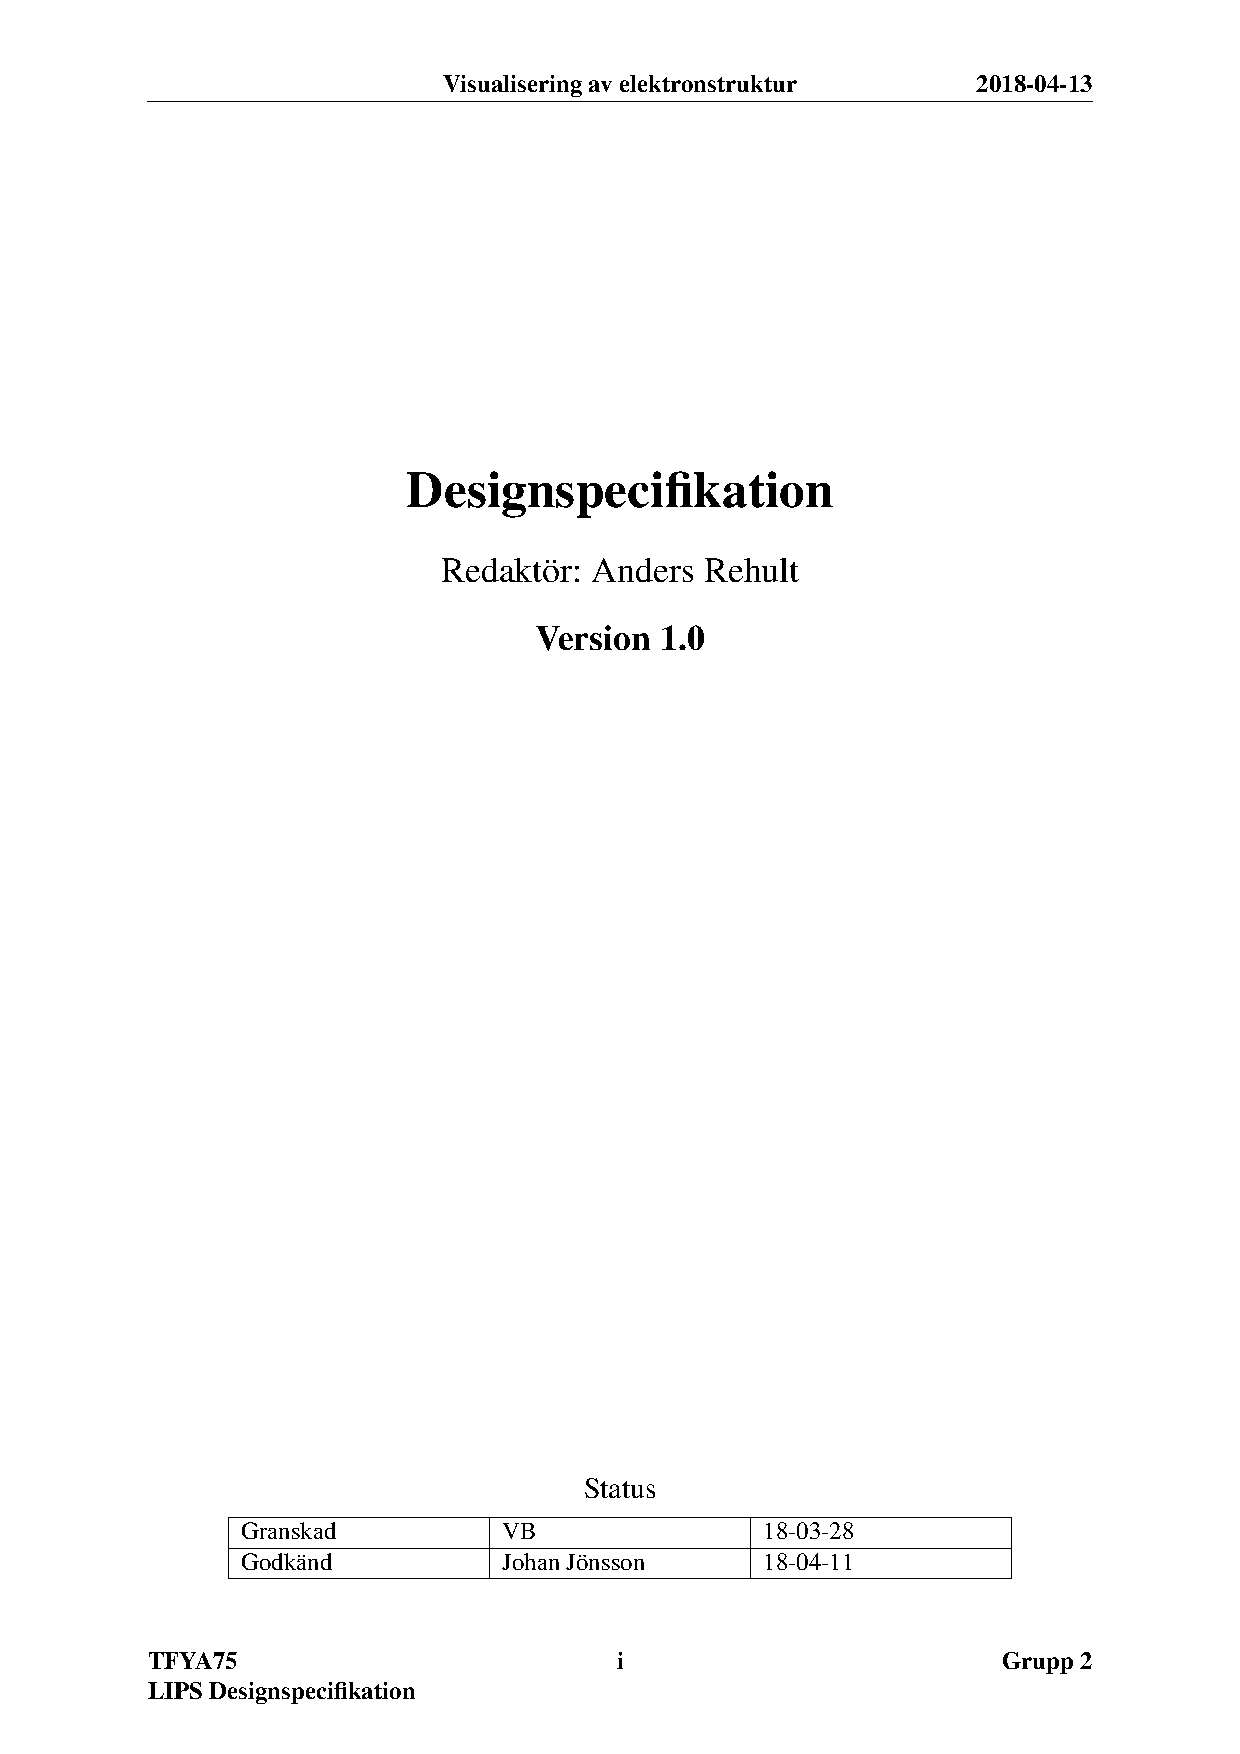
\includepdf[pages={1},pagecommand=\section{Designspecifikation}\label{appendix:designspecifikation}\thispagestyle{empty}]{designspecifikation_10.pdf}
\includepdf[pages={2-}]{designspecifikation_10.pdf}


\section{Fördjupningsarbete - Fermi-ytor}
\label{appendix:fermi-ytor}

\section{Fördjupningsarbete - Visualisering av volymdata}
\label{appendix:visualisering}


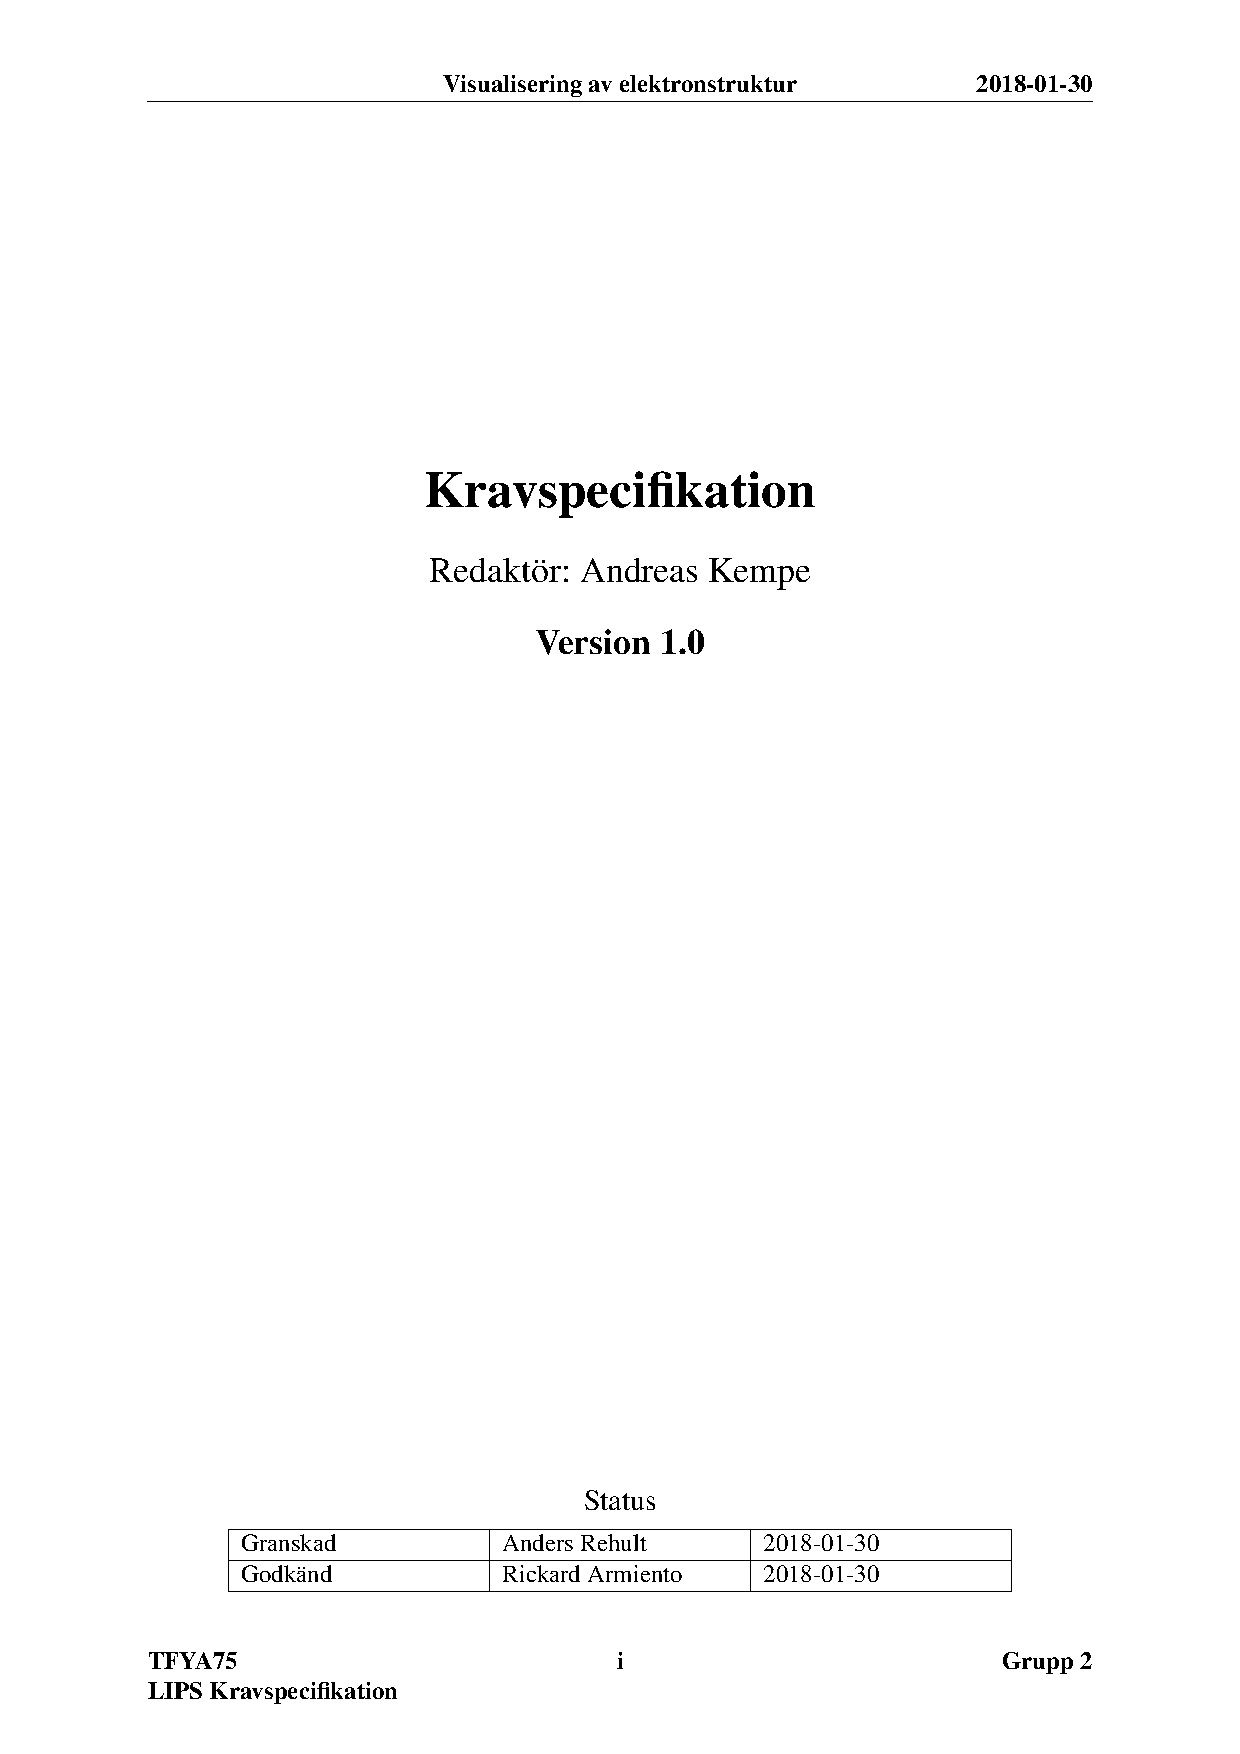
\includepdf[pages={1},pagecommand=\section{Kravspecifikation}\label{appendix:kravspecifikation}\thispagestyle{empty}]{Kravspecifikation_10.pdf}
\includepdf[pages={2-}]{Kravspecifikation_10.pdf}

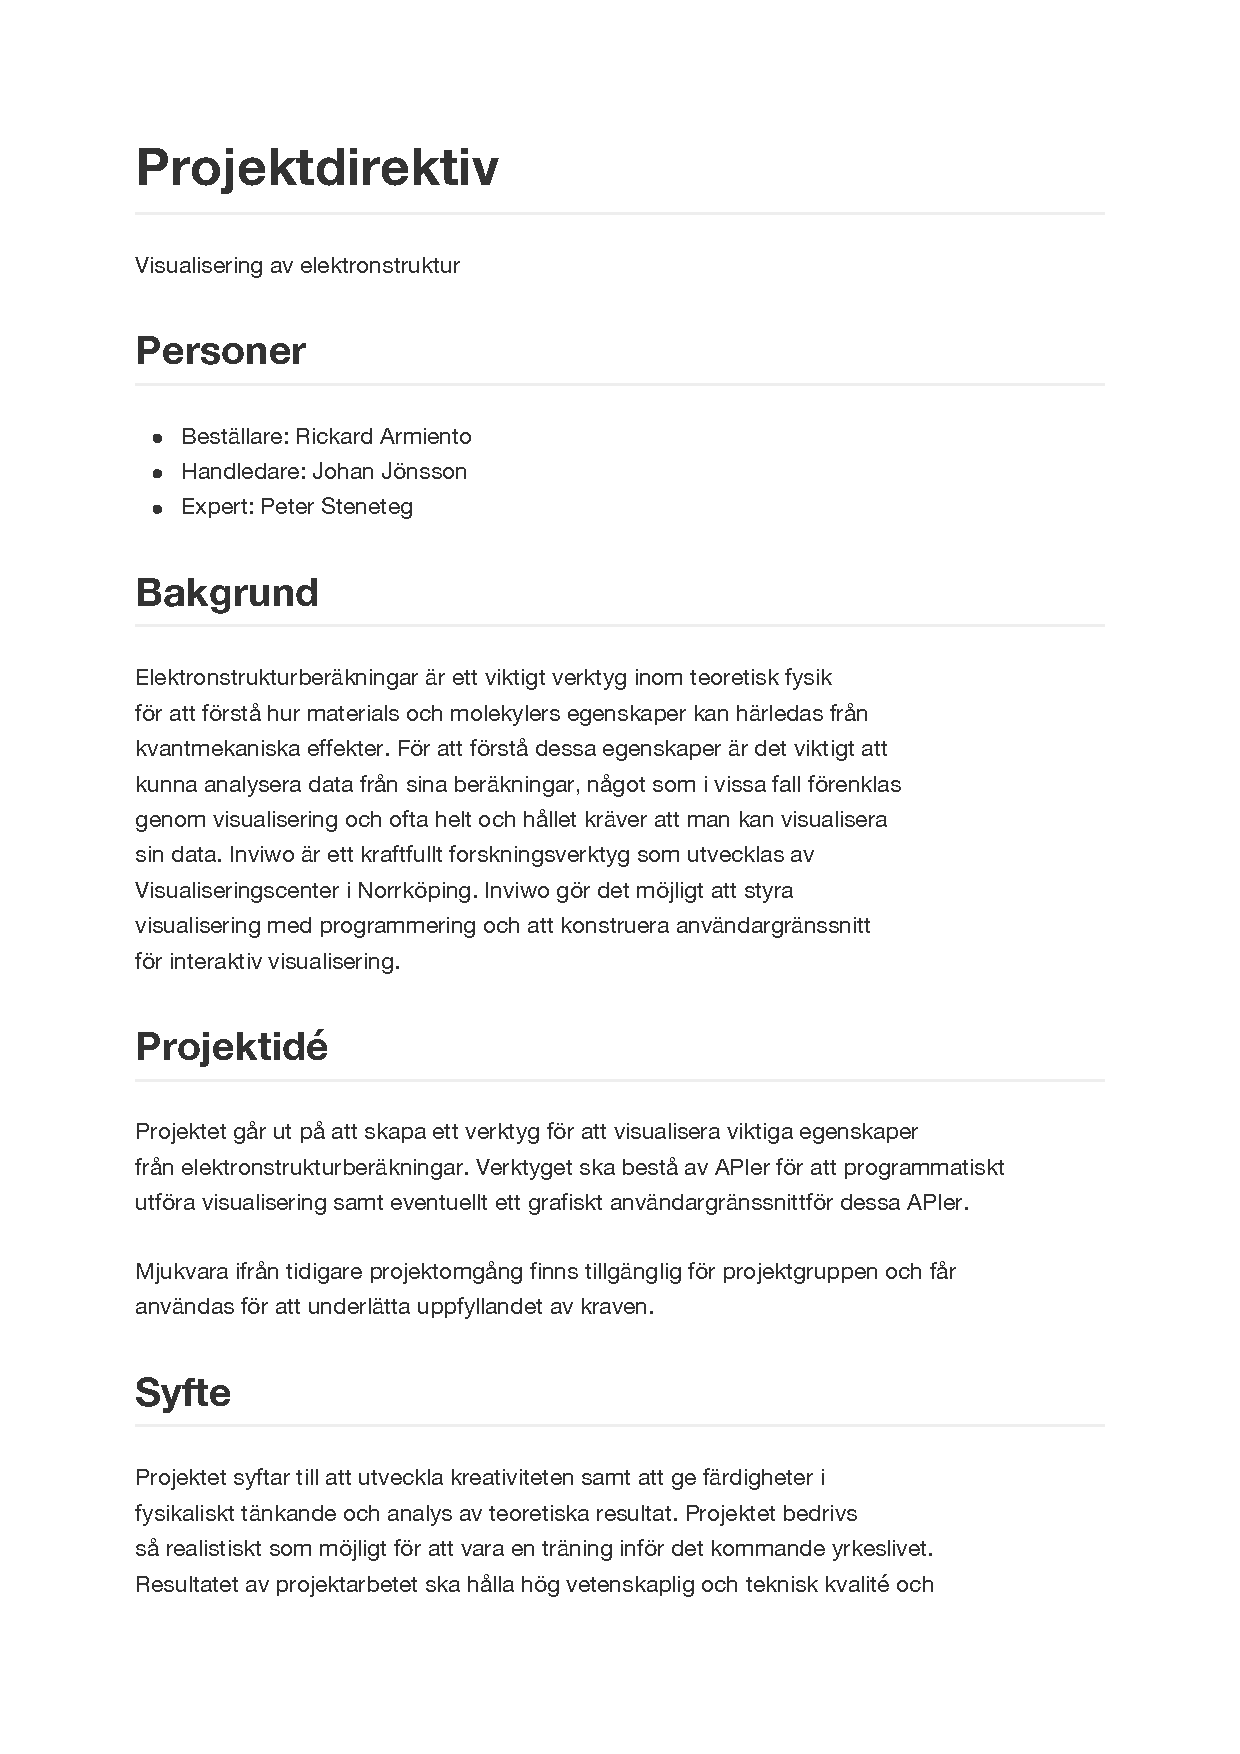
\includepdf[pages={1},pagecommand=\section{Projektdirektiv}\label{appendix:projektdirektiv}\thispagestyle{empty}]{projektdirektiv.pdf}
\includepdf[pages={2-}]{projektdirektiv.pdf}

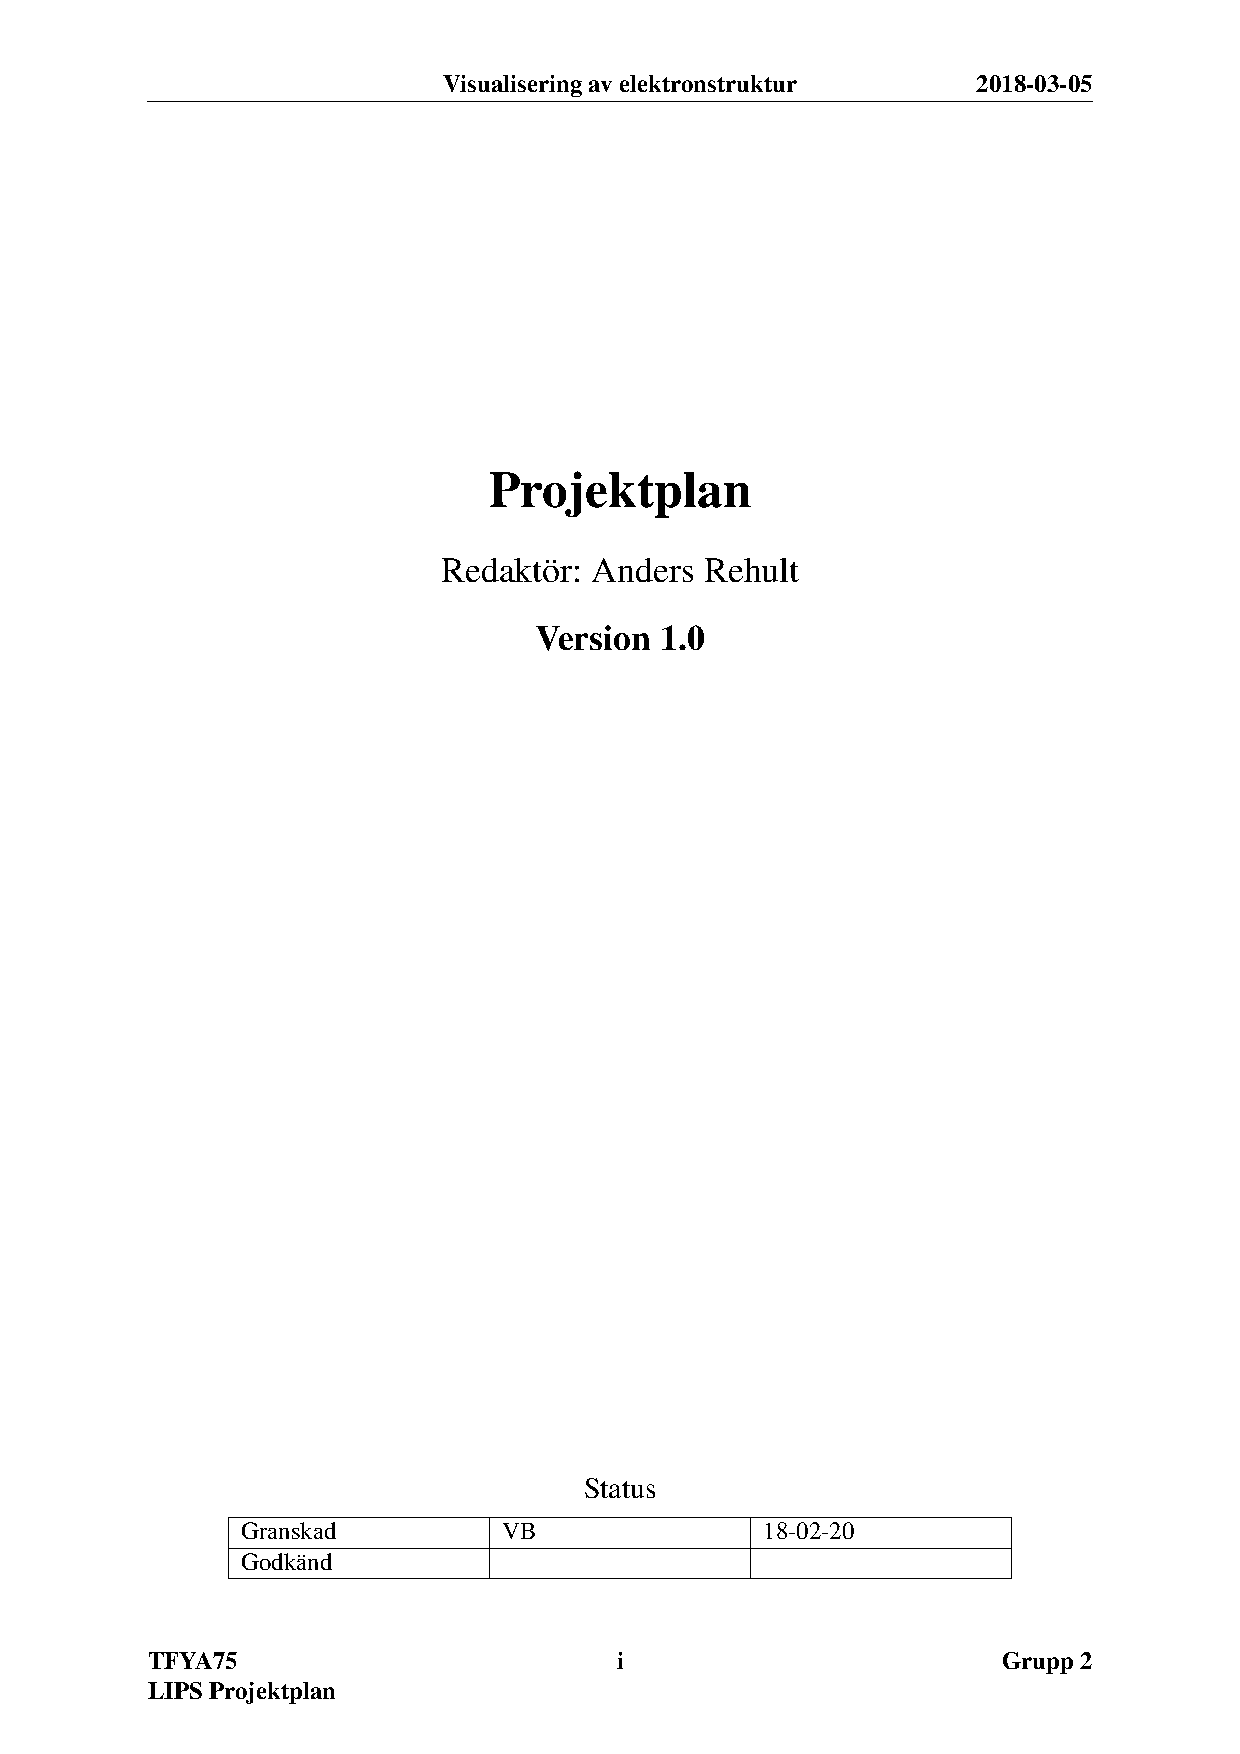
\includepdf[pages={1},pagecommand=\section{Projektplan}\label{appendix:projektplan}\thispagestyle{empty}]{projektplan_10.pdf}
\includepdf[pages={2-}]{projektplan_10.pdf}

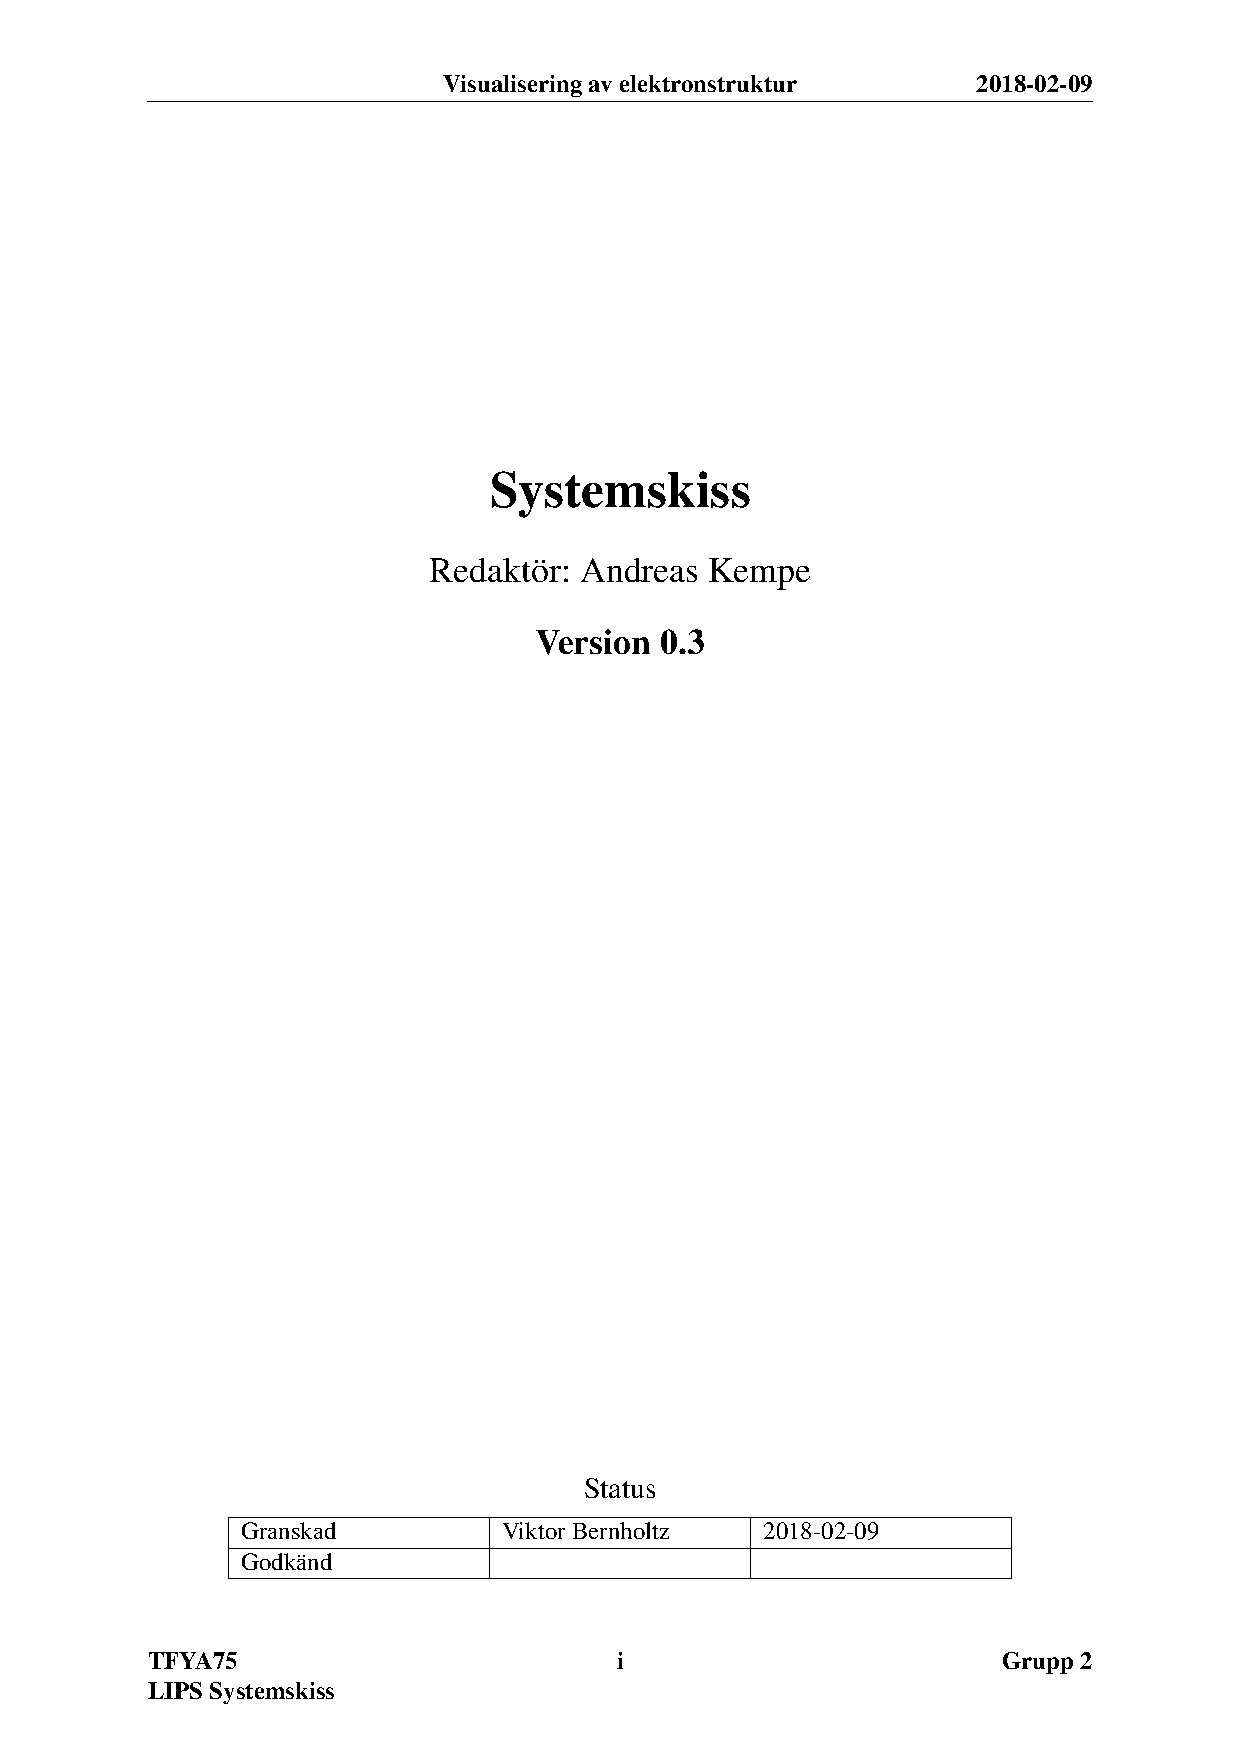
\includepdf[pages={1},pagecommand=\section{Systemskiss}\label{appendix:systemskiss}\thispagestyle{empty}]{Systemskiss_03.pdf}
\includepdf[pages={2-}]{Systemskiss_03.pdf}


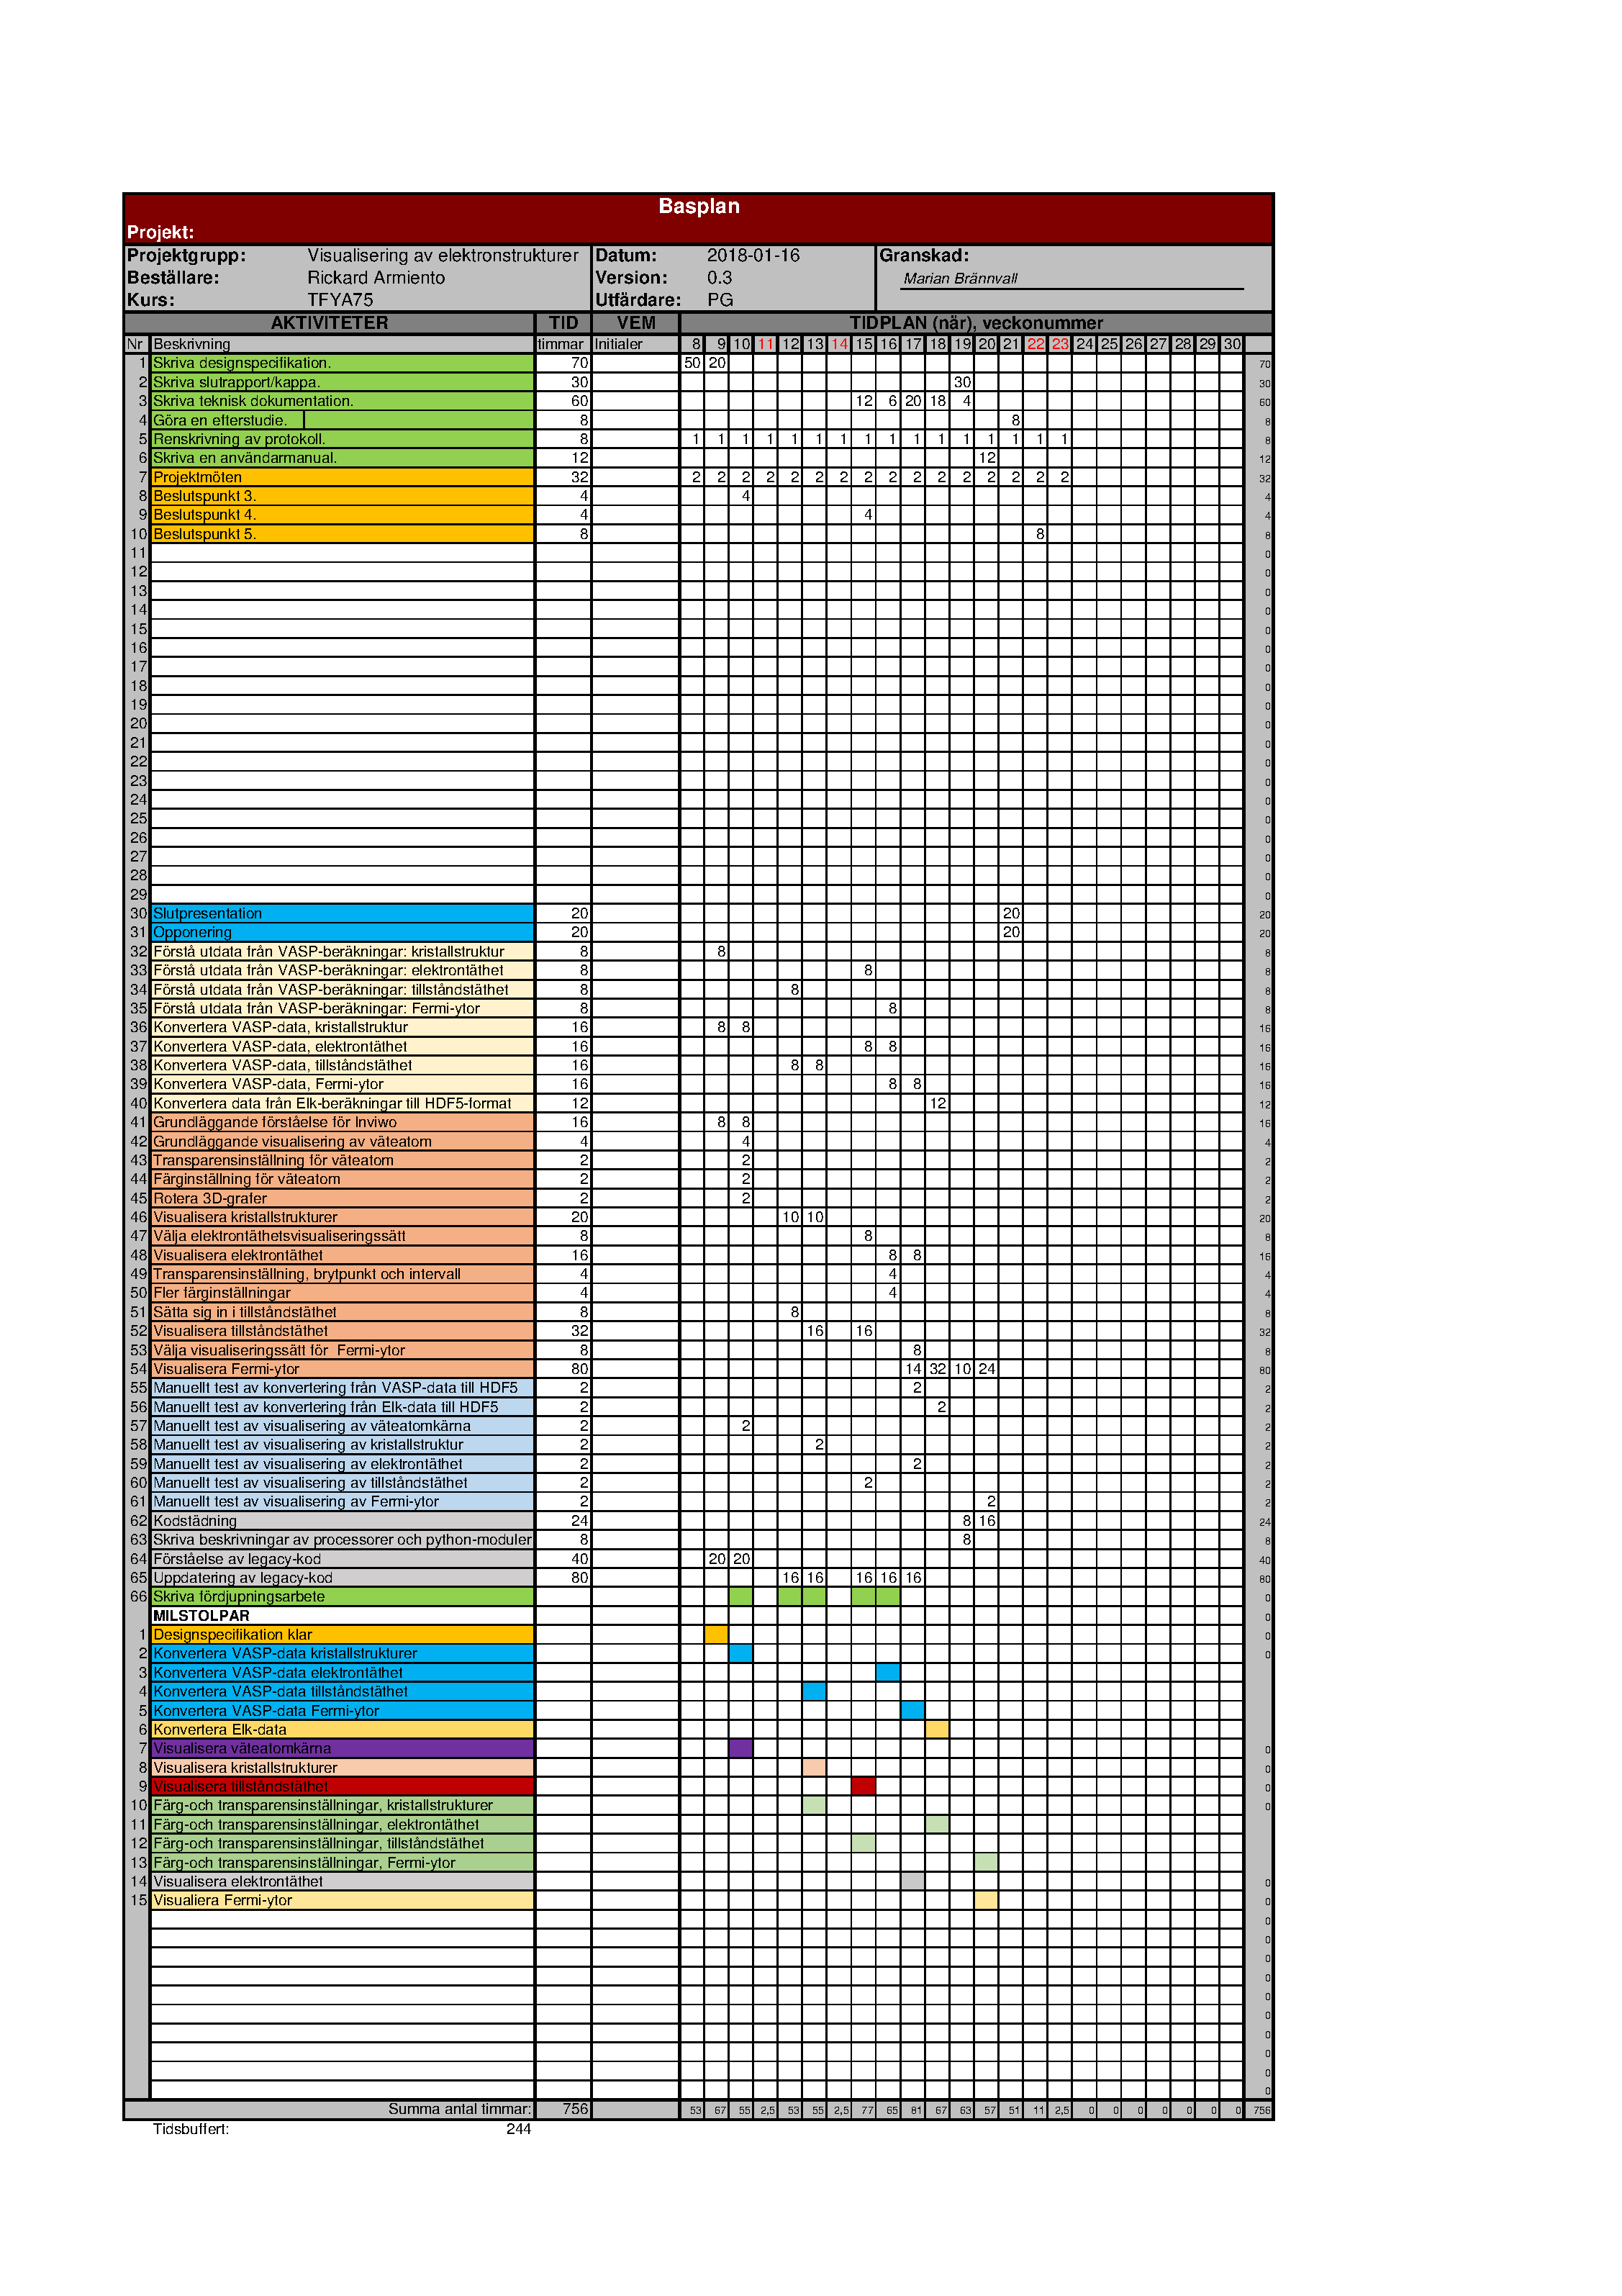
\includepdf[pages={1},pagecommand=\section{Tidplan}\label{appendix:tidplan}\thispagestyle{empty}]{tidplan_03.pdf}

\section{Teknisk dokumentation}
\label{appendix:teknisk-dokumentation}


\end{appendices}

\end{document} 
